\documentclass[11pt,a4paper]{article} 
\usepackage[portuges]{babel}
\usepackage[utf8]{inputenc}
\usepackage{graphicx}
\usepackage{pdflscape}
\usepackage{listings}
%\renewcommand{\lstlistingname}{Algoritmo} 
\usepackage{amsthm}
\usepackage{booktabs}
\usepackage{amsfonts}
\usepackage{subcaption}
\newtheorem{lema}{Lema}
\newtheorem{corolario}{Corolario}
\newtheorem{teorema}{Teorema}
\graphicspath{{images//}}

\title{Relatório - Trabalho 3 \\ Fecho convexo}
\author{Ronald A. Kaiser}


\begin{document}
    \maketitle

    \paragraph{}
    O objetivo deste trabalho é apresentar os algoritmos implementados para o problema do fecho convexo, juntamente com uma análise de seus desempenhos. Foram implementados os algoritmos de Jarvis, Graham e Andrew's Monotone Chain (variante do Graham).

    \section{Implementação}
    \paragraph{}
    O problema do fecho convexo pode ser resumido como encontrar o menor polígono convexo\footnote{Por menor polígono, entende-se o polígono com a menor quantidade de vértices possível.} que contém todos os pontos dados como entrada. Os algoritmos implementados recebem como entrada um conjunto de pontos V e retornam um conjunto de pontos $H \subseteq V$, acompanhado de sua ordenação em sentido anti-horário que pode ser usada para reconstruir o polígono do fecho convexo. 

    \paragraph{}
    Todos os algoritmos implementados se utilizam de uma primitiva básica para decidir se dois vetores estão dispostos em sentido horário ou anti-horário. Decidir se um vetor está à esquerda ou à direita de outro pode ser feito observando-se o sinal do produto vetorial dos dois vetores em questão. Esta primitiva é conhecida como teste CCW.

    \subsection{Jarvis}
    \paragraph{}
    O algoritmo de Jarvis foi desenvolvido em 1972 por R. A. Jarvis e também é conhecido como Gift Wrapping algorithm. Sua principal ideia é a cada iteração localizar o próximo vértice que compõe o fecho convexo de tal maneira a "embrulhar" os outros vértices. Como sabemos como identificar a posição relativa de dois vetores, basta a cada iteração varrer a lista de pontos procurando aquele ponto que está à esquerda de todos os outros. Paramos nossa busca quando encontramos o vértice pelo qual começamos a varredura.

    \subsection{Graham}
    \paragraph{}
    O algoritmo de Graham utiliza o teste CCW para ordenar os pontos por suas coordenadas polares em relação a um pivô (como pivô foi escolhido aquele com menor coordenada y). Uma vez concluída a ordenação, percorre-se os vértices naquela ordem para descobrirmos os vértices que farão parte do fecho. A cada iteração, quando encontramos um vértice que faz uma "curva para a direita", descartamos o anterior, dado que uma concavidade indesejada foi provocada por ele.

    \subsection{Andrew}
    \paragraph{}
    O algoritmo de Andrew's Monotone chain é considerado uma variante do algoritmo de Graham descrito acima. Também utiliza um processo de ordenação, mas nesta variante, não ordenamos em relação aos ângulos, e sim em relação às coordenadas x de cada ponto. A ideia é fazer duas passagens nos pontos de entrada. Uma vez da esquerda para a direita, definindo a envolvente inferior. E outra, da direita para a esquerda, construindo a envolvente superior. Ao final, concatenamos as duas soluções para compor a solução do problema original.

\clearpage
    \section{Testes}
    \paragraph{}
    Para testar os algoritmos implementados foi utilizado o seguinte conjunto de pontos como entrada:

        \begin{table}[!htb]
        \tiny
        \centering
        \caption{Entrada teste}
        \label{my-label}
        \begin{tabular}{l|l|l|l|l|l|l|l|l|l|l|l|l|l|l|l|l|l}
        \\\hline
        & A& B  & C & D & E  & F  & G & H & I & J  & K  & L  & M  & N  & O  & P  & Q    \\
        x & 3 & 11 & 6 & 4 & 5  & 8  & 1 & 7 & 9 & 14 & 10 & 17 & 15 & 13 & 3  & 12 & 16 \\
        y & 9 & 1  & 8 & 3 & 15 & 11 & 6 & 4 & 7 & 5  & 13 & 14 & 2  & 16 & 12 & 10 & 8  \\
        &   &    &   &   &    &    &   &   &   &    &    &    &    &    &    &    &                           
        \\\hline
            \end{tabular}
            \end{table}

    \paragraph{}
    Todos os algoritmos implementados geraram a mesma solução. A única diferença encontrada foi quanto à ordenação dos pontos da solução. Apesar de todos representarem a mesma solução em sentido anti-horário, o ponto de partida nem sempre coincidiam. Por exemplo, para a execução do Jarvis, a solução encontrada foi: B, M, L, N, E, O, G, D. Já para a execução do Andrew, a solução encontrada foi: G, D, B, M, L, N, E, O. Uma imagem da solução pode ser vista na figura~\ref{fig:sample}.
        \begin{figure}[htb]
            \captionsetup{justification=centering,margin=2cm}
            \centering
              \begin{minipage}[b]{0.4\textwidth}
              \centering
                  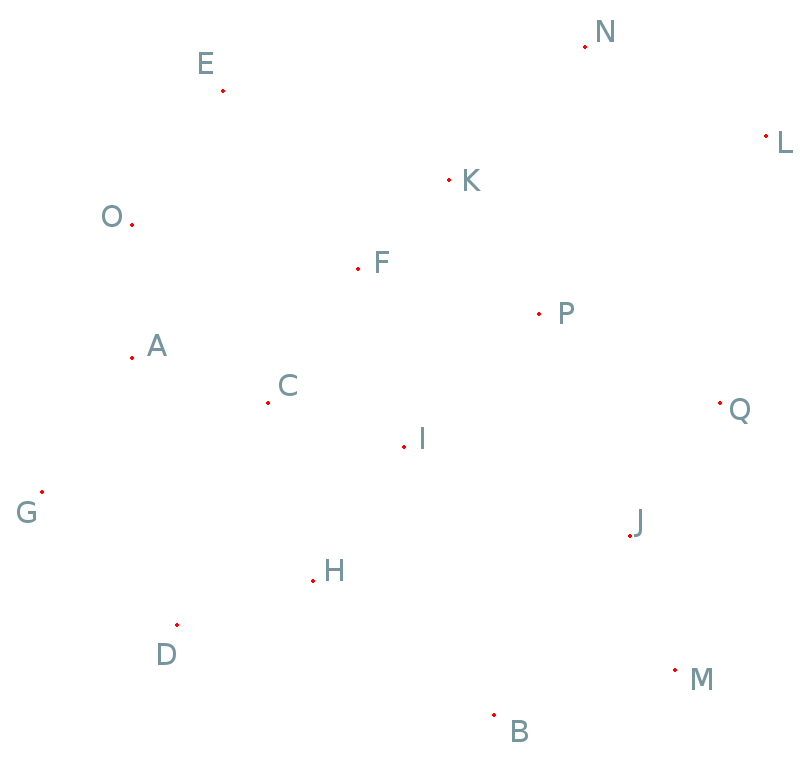
\includegraphics[width=.9\linewidth]{test_sample_input}
                  \subcaption{Input}
                \end{minipage}
                %
              \begin{minipage}[b]{0.4\textwidth}
              \centering
                  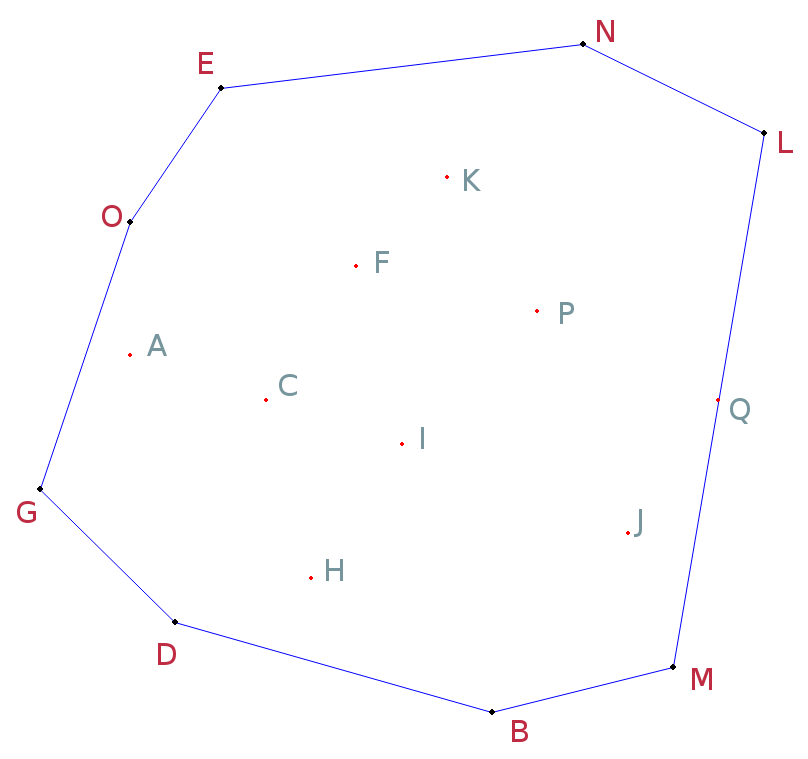
\includegraphics[width=.9\linewidth]{test_sample_ch}
                  \subcaption{Output}
                \end{minipage}
                \caption{Input/Output caso de teste.}
                \label{fig:sample}
        \end{figure}


    \paragraph{}
    Os grafos do trabalho anterior também foram utilizados para validar as implementações. Para o grafo das 128 cidades da América do Norte, o fecho convexo apresentou 13 vértices. Já para o grafo das sedes dos municípios do Brasil, o fecho apresentou 12 vértices. Nas figuras~\ref{fig:grafo1} e~\ref{fig:grafo2} são apresentadas as soluções.

        \begin{figure}[!htb]
          \begin{center}
              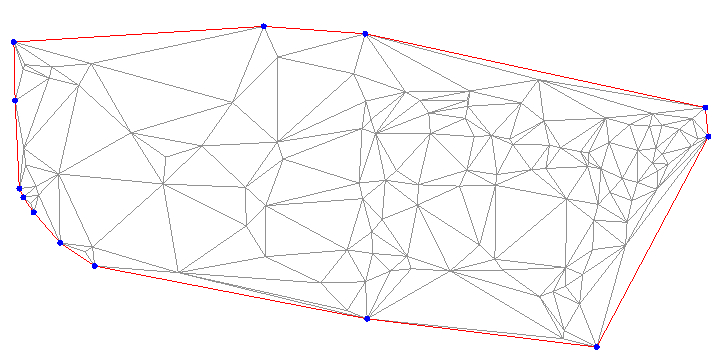
\includegraphics[scale=0.5]{america_ch}
          \end{center}
                \captionsetup{justification=centering,margin=2cm}
              \caption{Fecho convexo do grafo da América do Norte. Número de vértices do fecho: 13.}
              \label{fig:grafo1}
        \end{figure}

        \begin{figure}[!htb]
          \begin{center}
              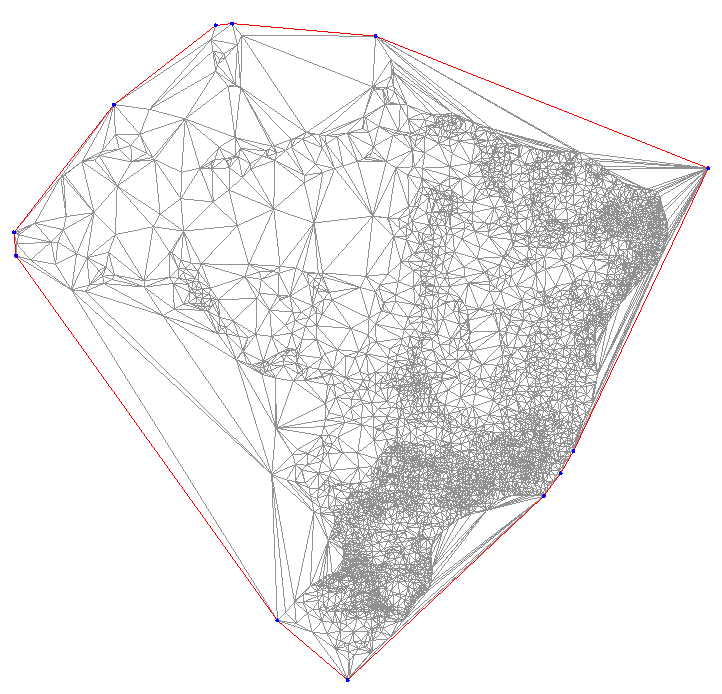
\includegraphics[scale=0.5]{brazil_ch}
          \end{center}
                \captionsetup{justification=centering,margin=2cm}
              \caption{Fecho convexo do grafo das sedes dos municípios do Brasil. Número de vértices do fecho: 12.}
              \label{fig:grafo2}
        \end{figure}


\clearpage
    \section{Desempenho}
    \paragraph{}
    Para analisar o desempenho dos algoritmos foram utilizadas amostras de conjuntos de pontos em configurações específicas. Foram considerados pontos dentro de um retângulo, triângulo\footnote{Para a geração dos pontos aleatórios dentro do triângulo foi utilizada a técnica descrita em: http://mathworld.wolfram.com/TrianglePointPicking.html}, círculo e sobre o círculo. 

        \begin{figure}[!htb]
                \captionsetup{justification=centering,margin=2cm}
            \centering
              \begin{minipage}[b]{0.2\textwidth}
              \centering
                  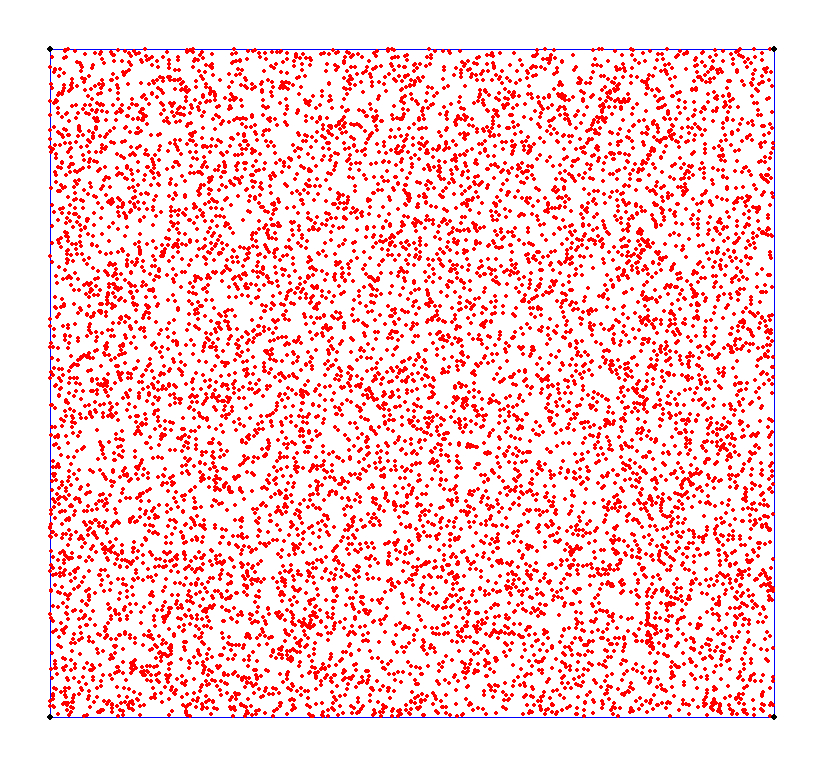
\includegraphics[width=.8\linewidth]{rectangle}
                  \label{fig:map}
                  %\subcaption{Exemplo de amostra com 10000 pontos no interior de um retângulo}
                \end{minipage}
                %
              \begin{minipage}[b]{0.2\textwidth}
              \centering
                  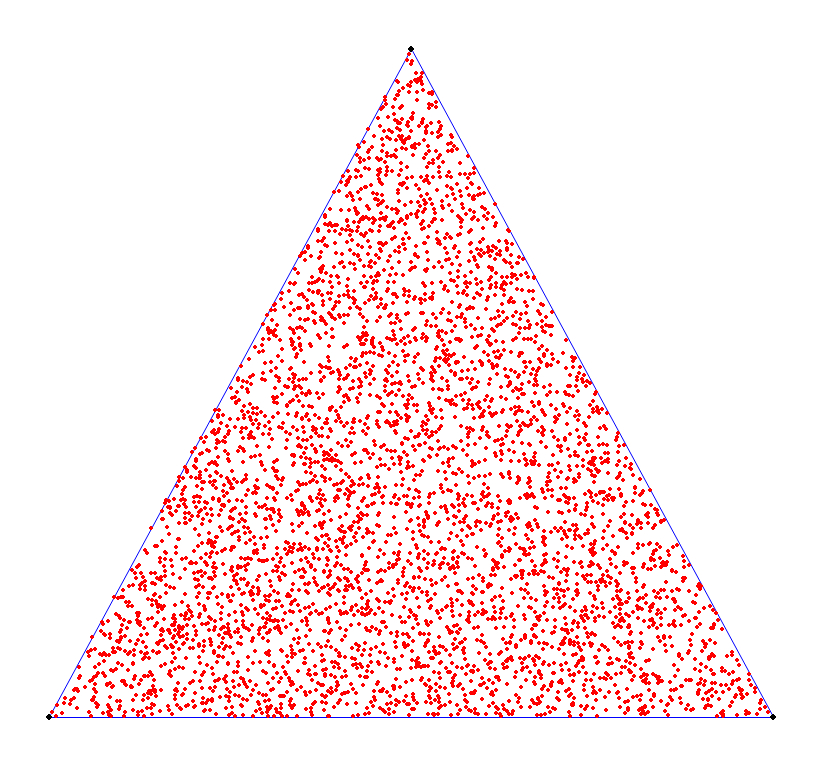
\includegraphics[width=.8\linewidth]{triangle}
                  \label{fig:map}
                  %\subcaption{Exemplo de amostra com 10000 pontos no interior de um triângulo}
                \end{minipage}
                %
              \begin{minipage}[b]{0.2\textwidth}
              \centering
                  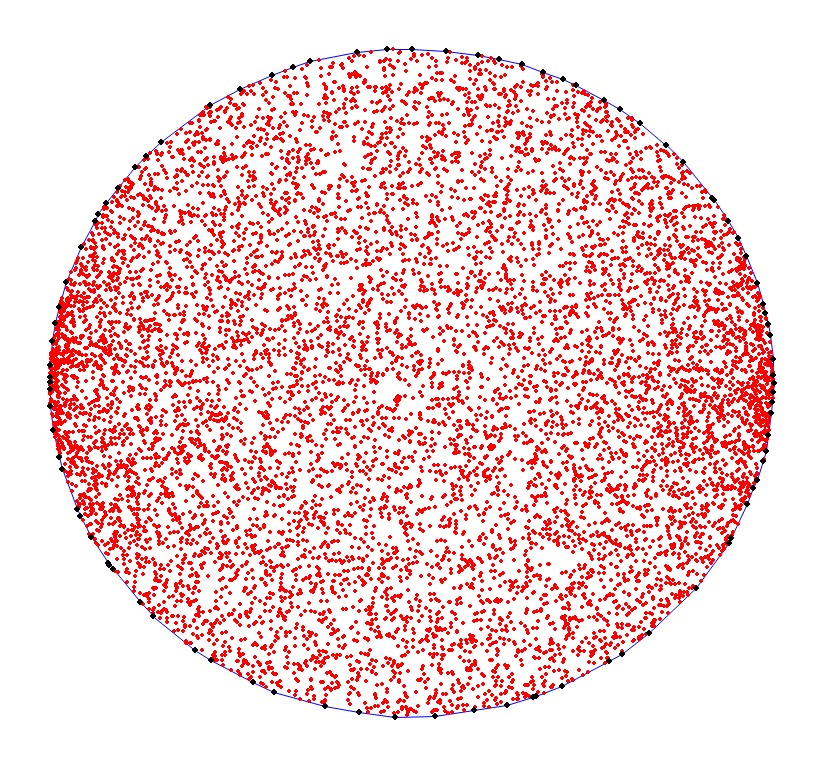
\includegraphics[width=.8\linewidth]{inside_circle}
                  \label{fig:map}
                  %\subcaption{Exemplo de amostra com 10000 pontos no interior de círculo}
                \end{minipage}
                %
              \begin{minipage}[b]{0.2\textwidth}
              \centering
                  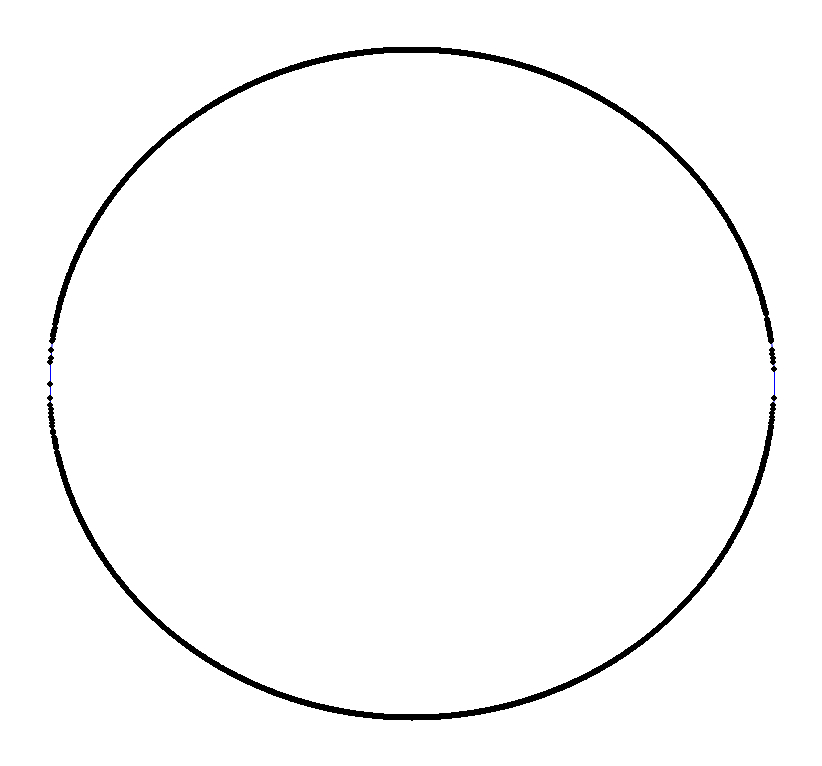
\includegraphics[width=.8\linewidth]{on_circle}
                  \label{fig:map}
                  %\subcaption{Exemplo de amostra com 10000 pontos sobre um círculo}
                \end{minipage}
                \caption{Configurações de pontos testadas.}
        \end{figure}

    \paragraph{}
    Em geral, o desempenho dos algoritmos de Graham e Andrew são parecidos (com a implementação do algoritmo de Andrew levando uma pequena vantagem), dado que são variantes e têm complexidade igual a $O(nlogn)$. Para a maior parte dos testes, o algoritmo de Jarvis demonstrou ser inferior ou equivalente aos outros dois.
    
    \paragraph{}
    Vale ressaltar que quando o número de pontos no fecho convexo é pequeno ($< log(n)$), o algoritmo de Jarvis tem desempenho melhor do que os outros, já que sua complexidade é $O(nh)$. Nos testes que envolvem pontos sobre o círculo, ele se sai muito pior do que os outros, pois, todos os pontos de entrada farão parte do fecho convexo, caso em que h = n e a complexidade se torna quadrática. Na figura~\ref{fig:vertices}, é possível observar, entretanto, o algoritmo de Jarvis obtendo um desempenho melhor quando adicionamos os vértices do retângulo e do triângulo. Quando adicionamos os vértices do triângulo, por exemplo, h = 3 e a complexidade do Jarvis se torna O(3n), enquanto que a do Graham se mantém em $O(nlogn)$.

    \paragraph{}
    Quanto ao esforço relativo à implementação, os algoritmos têm complexidade parecida. O Graham se apresentou um pouco mais complicado de implementar, pois exigia uma atenção maior aos casos de exceção de colinearidade. O algoritmo de Andrew acabou tendo a implementação mais simples de todos, e em geral se saiu melhor quanto ao desempenho.

        \begin{figure}[!htb]
                \captionsetup{justification=centering,margin=2cm}
            \centering
              \begin{minipage}[b]{\textwidth}
              \centering
                  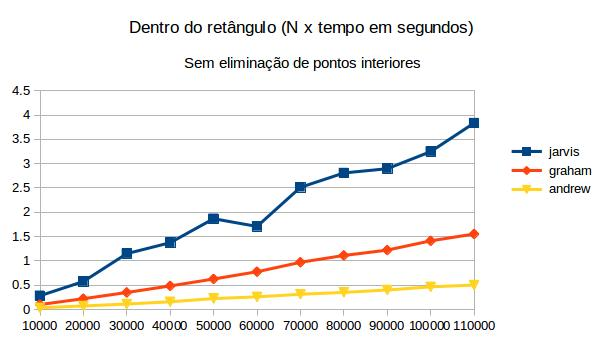
\includegraphics[width=\linewidth]{graph_retangulo_no}
                  \label{fig:map}
                \end{minipage}
                %
              \begin{minipage}[b]{\textwidth}
              \centering
                  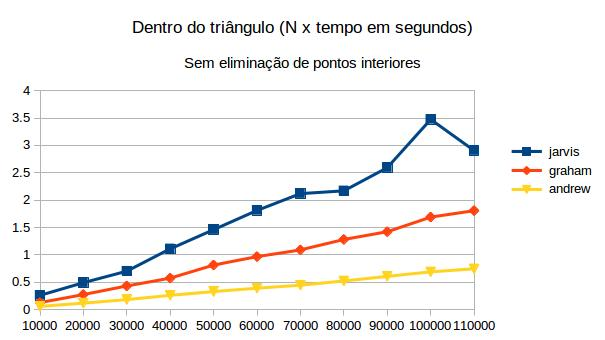
\includegraphics[width=\linewidth]{graph_triangulo_no}
                  \label{fig:map}
                \end{minipage}
                \caption{}
        \end{figure}

        \begin{figure}[!htb]
            \centering
              \begin{minipage}[b]{\textwidth}
              \centering
                  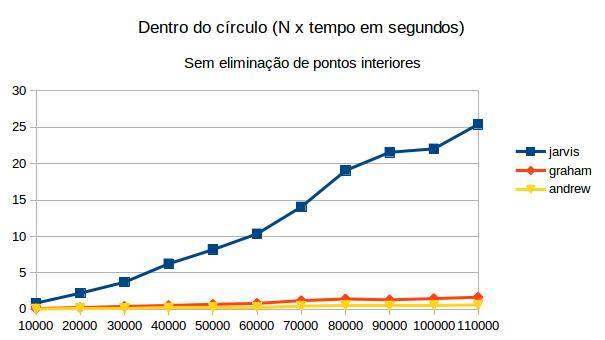
\includegraphics[width=\linewidth]{graph_circulo_no}
                  \label{fig:map}
                \end{minipage}
                %
              \begin{minipage}[b]{\textwidth}
              \centering
                  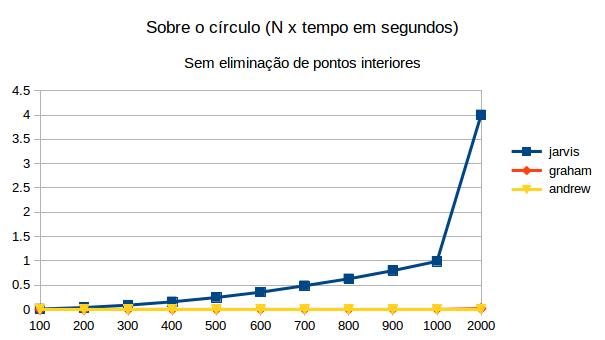
\includegraphics[width=\linewidth]{graph_sobre_circulo_no}
                  \label{fig:map}
                \end{minipage}
                \caption{}
                \label{fig:sem}
        \end{figure}


        \begin{figure}[!htb]
                \captionsetup{justification=centering,margin=2cm}
            \centering
              \begin{minipage}[b]{\textwidth}
              \centering
                  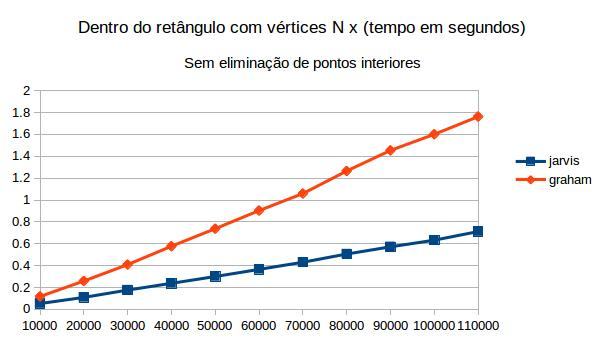
\includegraphics[width=\linewidth]{graph_vertices_retangulo_no}
                  \label{fig:map}
                \end{minipage}
                %
              \begin{minipage}[b]{\textwidth}
              \centering
                  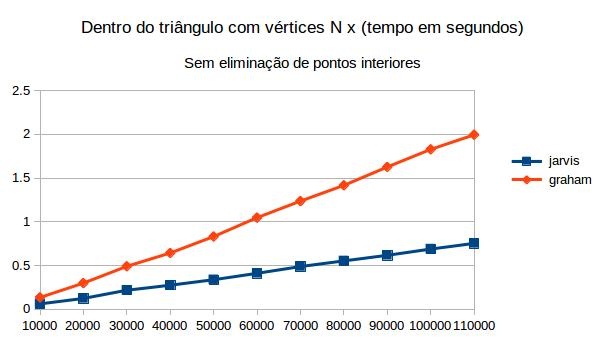
\includegraphics[width=\linewidth]{graph_vertices_triangulo_no}
                  \label{fig:map}
                \end{minipage}
                \caption{}
                \label{fig:vertices}
        \end{figure}


\clearpage
    \section{Eliminação de pontos interiores}
    \paragraph{}
    Os testes de desempenho realizados na seção anterior foram refeitos introduzindo eliminação de pontos interiores como estratégia para reduzir o conjunto de entrada e assim, diminuir o tempo de execução dos algoritmos.

    \paragraph{}
    A partir dos testes executados, na maioria dos casos a utilização de eliminação de pontos interiores melhorou o desempenho do algoritmo Jarvis. Nas configurações em que os pontos estavam dispostos dentro de um retângulo e dentro de um triângulo, os três algoritmos se tornaram praticamente equivalentes. Já para os pontos dentro de um círculo os tempos do Jarvis caíram praticamente pela metade. Só não houve melhoria no caso em que os pontos estavam sobre o círculo, caso em que a eliminação não tem efeito algum e constitui o pior caso do algoritmo Jarvis.

        \begin{figure}[!htb]
                \captionsetup{justification=centering,margin=2cm}
            \centering
              \begin{minipage}[b]{.8\textwidth}
              \centering
                  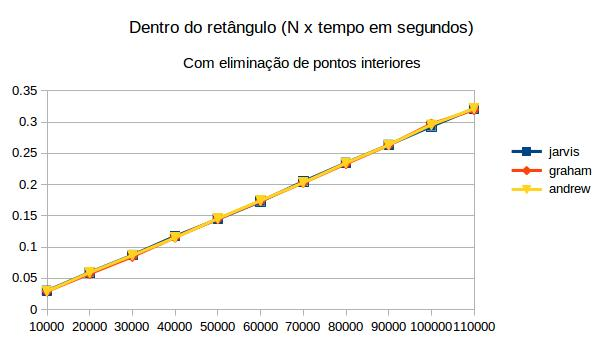
\includegraphics[width=\linewidth]{graph_retangulo_yes}
                  \label{fig:map}
                \end{minipage}
                %
              \begin{minipage}[b]{.8\textwidth}
              \centering
                  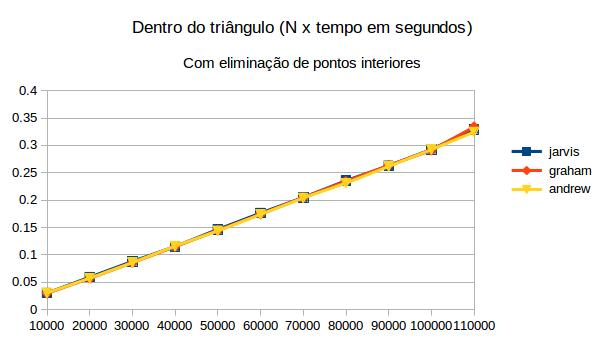
\includegraphics[width=\linewidth]{graph_triangulo_yes}
                  \label{fig:map}
                \end{minipage}
                \caption{}
            \end{figure}

            \begin{figure}[!htb]
              \begin{minipage}[b]{\textwidth}
              \centering
                  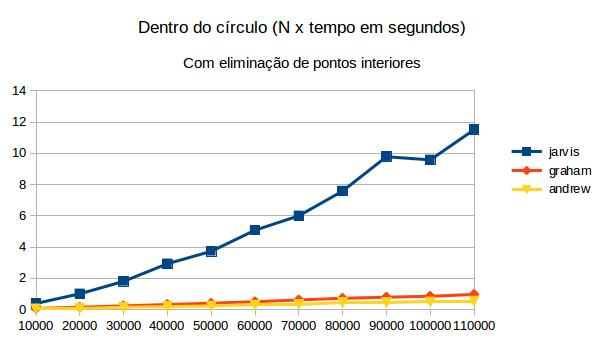
\includegraphics[width=\linewidth]{graph_circulo_yes}
                  \label{fig:map}
                \end{minipage}
                %
              \begin{minipage}[b]{\textwidth}
              \centering
                  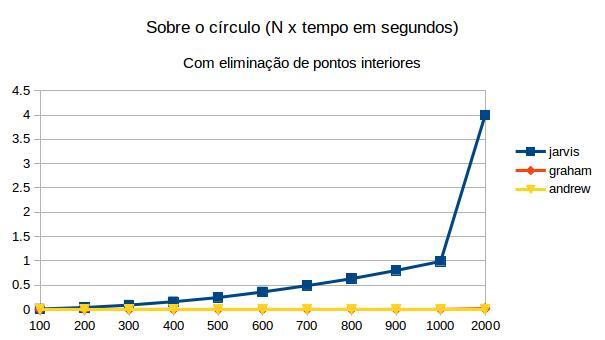
\includegraphics[width=\linewidth]{graph_sobre_circulo_yes}
                  \label{fig:map}
                \end{minipage}
                \caption{}
        \end{figure}

        \paragraph{}
        Foi executado um profiling sobre o código para entendermos melhor onde se dá a maior parte do processamento e qual fração do tempo está sendo utilizada no cálculo da eliminação dos pontos interiores. Como exemplo, utilizamos a entrada do Grafo Brasil no algoritmo de Jarvis e Graham.

        \subsection{Jarvis profiling}
        \paragraph{}
        É possível perceber no código a seguir que a maior parte do tempo de execução se dá varrendo os pontos e executando testes CCW. Repare que no primeiro código, não foi utilizada eliminação de pontos interiores e o tempo total de execução foi de aproximadamente 0.41s. No entanto, no segundo, foi utilizada eliminação de pontos, gastando um total de $15\%$ do tempo de execução total, mas ainda assim, o tempo total de execução foi de ~0.27s, representando assim, uma evidente vantagem no uso de eliminação de pontos interiores.

        \paragraph{}
        Os casos em que não se verifica uma vantagem são aqueles em que eliminamos uma fração muito pequena de pontos, e o custo de eliminá-los acaba causando um overhead sobre a execução. Mas como a eliminação tem custo O(n), e para este problema precisamos ao menos ler a entrada ($\Omega(n)$), na média, representa uma vantagem aplicar tal eliminação.

        \subsection{Graham profiling}
        \paragraph{}
        No algoritmo de Graham o processo de ordenação representa o maior custo computacional. Com a adição da eliminação de pontos interiores, o custo total diminuiu, apesar da eliminação de pontos causar um overhead inicial.

\lstset{
  basicstyle=\fontsize{6}{6}\selectfont\ttfamily
}
\begin{landscape}
\begin{lstlisting}[language=Python]
Total time: 0.409528 s
File: jarvis.py
Function: jarvis at line 31

Line #      Hits         Time  Per Hit   % Time  Line Contents
==============================================================
    31                                           @profile
    32                                           def jarvis(points, cutoff=False):
    33         2            3      1.5      0.0      if cutoff: points = interior_elimination(points)
    34         2         1501    750.5      0.4      pts = list(set(points))
    35         2         4177   2088.5      1.0      P0 = min(pts, key=lambda p: (p[1], p[0]))
    36         2            3      1.5      0.0      H = [P0]
    37                                               
    38        26           19      0.7      0.0      for h in H:
    39        24           19      0.8      0.0          a = h 
    40    133584        76293      0.6     18.6          for b in pts:
    41    133560       327091      2.4     79.9              if ccw(h, a, b) < 0 or (ccw(h, a, b) == 0 and \
    42        48          175      3.6      0.0                  distance(h, b) > distance(h, a)):
    43       246          149      0.6      0.0                  a = b
    44        24            9      0.4      0.0          if a is not P0:
    45        22           34      1.5      0.0              H.append(a)
    46                                           
    47         2           53     26.5      0.0      assert is_convex(H)
    48         2            2      1.0      0.0      return H
\end{lstlisting}


\begin{lstlisting}[language=Python]
Total time: 0.272519 s
File: jarvis.py
Function: jarvis at line 31

Line #      Hits         Time  Per Hit   % Time  Line Contents
==============================================================
    31                                           @profile
    32                                           def jarvis(points, cutoff=False):
    33         2        39749  19874.5     14.6      if cutoff: points = interior_elimination(points)
    34         2          891    445.5      0.3      pts = list(set(points))
    35         2         2342   1171.0      0.9      P0 = min(pts, key=lambda p: (p[1], p[0]))
    36         2            3      1.5      0.0      H = [P0]
    37                                               
    38        26           16      0.6      0.0      for h in H:
    39        24            9      0.4      0.0          a = h 
    40     75576        44260      0.6     16.2          for b in pts:
    41     75552       184838      2.4     67.8              if ccw(h, a, b) < 0 or (ccw(h, a, b) == 0 and \
    42        48          156      3.2      0.1                  distance(h, b) > distance(h, a)):
    43       228          154      0.7      0.1                  a = b
    44        24           16      0.7      0.0          if a is not P0:
    45        22           33      1.5      0.0              H.append(a)
    46                                           
    47         2           50     25.0      0.0      assert is_convex(H)
    48         2            2      1.0      0.0      return H
\end{lstlisting}

\clearpage

\begin{lstlisting}[language=Python]
Total time: 0.30633 s
File: graham.py
Function: graham at line 37

Line #      Hits         Time  Per Hit   % Time  Line Contents
==============================================================
    37                                           @profile
    38                                           def graham(points, cutoff=False):
    39         2            4      2.0      0.0      if cutoff: points = interior_elimination(points)
    40         2         1536    768.0      0.5      pts = list(set(points)) 
    41                                           
    42         2         4098   2049.0      1.3      P0 = min(pts, key=lambda p: (p[1], p[0]))
    43         2          291    145.5      0.1      pts.remove(P0)
    44                                           
    45         2            2      1.0      0.0      to_ignore = {}
    46         2       218308 109154.0     71.3      pts.sort(lambda B, C: compare(P0, B, C, to_ignore))
    47                                           
    48         2           11      5.5      0.0      H = [P0] + pts[:2]
    49                                           
    50     11126         8853      0.8      2.9      for i in range(2, len(pts)):
    51     11124        10123      0.9      3.3          if pts[i] in to_ignore: continue
    52     22230        42294      1.9     13.8          while ccw(H[-2], H[-1], pts[i]) <= 0:
    53     11106        10213      0.9      3.3              H.pop()
    54     11124        10548      0.9      3.4          H.append(pts[i])
    55                                           
    56         2           47     23.5      0.0      assert is_convex(H)
    57         2            2      1.0      0.0      return H
\end{lstlisting}

\begin{lstlisting}[language=Python]
Total time: 0.21002 s
File: graham.py
Function: graham at line 37

Line #      Hits         Time  Per Hit   % Time  Line Contents
==============================================================
    37                                           @profile
    38                                           def graham(points, cutoff=False):
    39         2        39923  19961.5     19.0      if cutoff: points = interior_elimination(points)
    40         2          874    437.0      0.4      pts = list(set(points)) 
    41                                           
    42         2         2462   1231.0      1.2      P0 = min(pts, key=lambda p: (p[1], p[0]))
    43         2          163     81.5      0.1      pts.remove(P0)
    44                                           
    45         2            2      1.0      0.0      to_ignore = {}
    46         2       121029  60514.5     57.6      pts.sort(lambda B, C: compare(P0, B, C, to_ignore))
    47                                           
    48         2            7      3.5      0.0      H = [P0] + pts[:2]
    49                                           
    50      6292         4814      0.8      2.3      for i in range(2, len(pts)):
    51      6290         5542      0.9      2.6          if pts[i] in to_ignore: continue
    52     12562        23805      1.9     11.3          while ccw(H[-2], H[-1], pts[i]) <= 0:
    53      6272         5574      0.9      2.7              H.pop()
    54      6290         5780      0.9      2.8          H.append(pts[i])
    55                                           
    56         2           44     22.0      0.0      assert is_convex(H)
    57         2            1      0.5      0.0      return H
\end{lstlisting}

\end{landscape}



\clearpage
    \section{Ordenação}
    \paragraph{}
    Como dito anteriormente, os algoritmos de Graham e Andrew utilizam um procedimento de ordenação numa primeira etapa, que representa o maior custo destes algoritmos. Após este procedimento, os dois algoritmos prosseguem com custo linear varrendo os pontos na ordem previamente definida. Substituir os algoritmos de ordenação de complexidade nlogn por outros de complexidade quadrática, faria com que os algoritmos Graham e Andrew passassem a ter complexidade assintótica também quadrática.




\end{document}
